\subsubsection{Package della componente View}
	\begin{figure}[h!]
	\begin{center}
		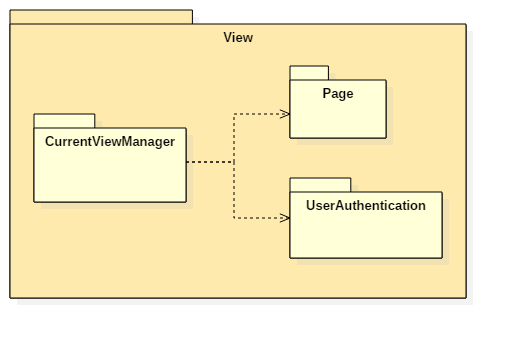
\includegraphics[scale=0.6]{../images/ViewPackage.png}
		\caption{Package della componente View}
	\end{center}
	\end{figure}
	Il package per il componente View del pattern architetturale MVP contiene i seguenti sotto packages:
	\begin{itemize}
		\item\textbf{CurrentViewManager:} questo sotto package ha lo scopo di definire lo stato attuale del sistema Quizzipedia; per fare ciò si avvale delle classi:
			\begin{itemize}
				\item\textit{CurrentView}%mettere link alla sezione in cui è spiegata
				\item\textit{Sender}%mettere link alla sezione in cui è spiegata
			\end{itemize}
		\item\textbf{Pages:} contiene la classe astratta \textit{Page}, che rappresenta una specifica situazione del sistema (ovvero una pagina web del sito), più tutte le sue derivazioni concrete:
			\begin{itemize}
				\item\textit{MainPage}%mettere link alla sezione in cui è spiegata
				\item\textit{CategoryListPage}%mettere link alla sezione in cui è spiegata
				\item\textit{QuizListPage}%mettere link alla sezione in cui è spiegata
				\item\textit{QuizExecutionPage}%mettere link alla sezione in cui è spiegata
				\item\textit{QuizManagementPage}%mettere link alla sezione in cui è spiegata
				\item\textit{ViewTutorialPage}%mettere link alla sezione in cui è spiegata
			\end{itemize}
		\item\textbf{UserAuthentication:} contiene la classe \textit{User} che raggruppa le funzionalità di autenticazione di un utente generico sulla piattaforma Quizzipedia; come \textit{Pages} anche \textit{UserAuthentication} è un package d'appoggio per la classe \textit{CurrentViewManager}::\textit{CurrentView}.\\
		\\
	\end{itemize}	